This chapter provides detailed specifications of the system under development.

\section{Functional Requirements}
\begin{outline}
  \1 Authorization / Authentication:
  \2 To allow the user to sign up using the QR code provided in the booklet.
  \2 To allow the user to keep record of their progress to the cloud.
  \2 To allow the user to fetch progress data from the cloud each time the app starts.
  \1 Augmented Reality:
  \2 To identify physical markers from the booklet.
  \2 To render 3D models, simulations, and games on top of the identified markers.
  \2 To take touch input as a means of interaction between the user and the simulations/models.
\end{outline}

% --- The above is to be modified as per your project, e.g. a flat list if your system has limited functional requirements.

\section{Non-functional Requirements}
\begin{outline}
  \1 Performance:
  \2 The app should be able to smoothly render 3D models and simulations, ideally, without lag.
  \2 There should be minimal lag in the user interacting using touch and the model / simulation responding to it.
  \1 Availability:
  \2 The app should be readily available on compatible platform-specific app store(s).
  \1 Deployment:
  \2 The app should be deployed on an app store that ensures reliable public access.
\end{outline}

\section{External Interfaces}
\subsection{User Interfaces}
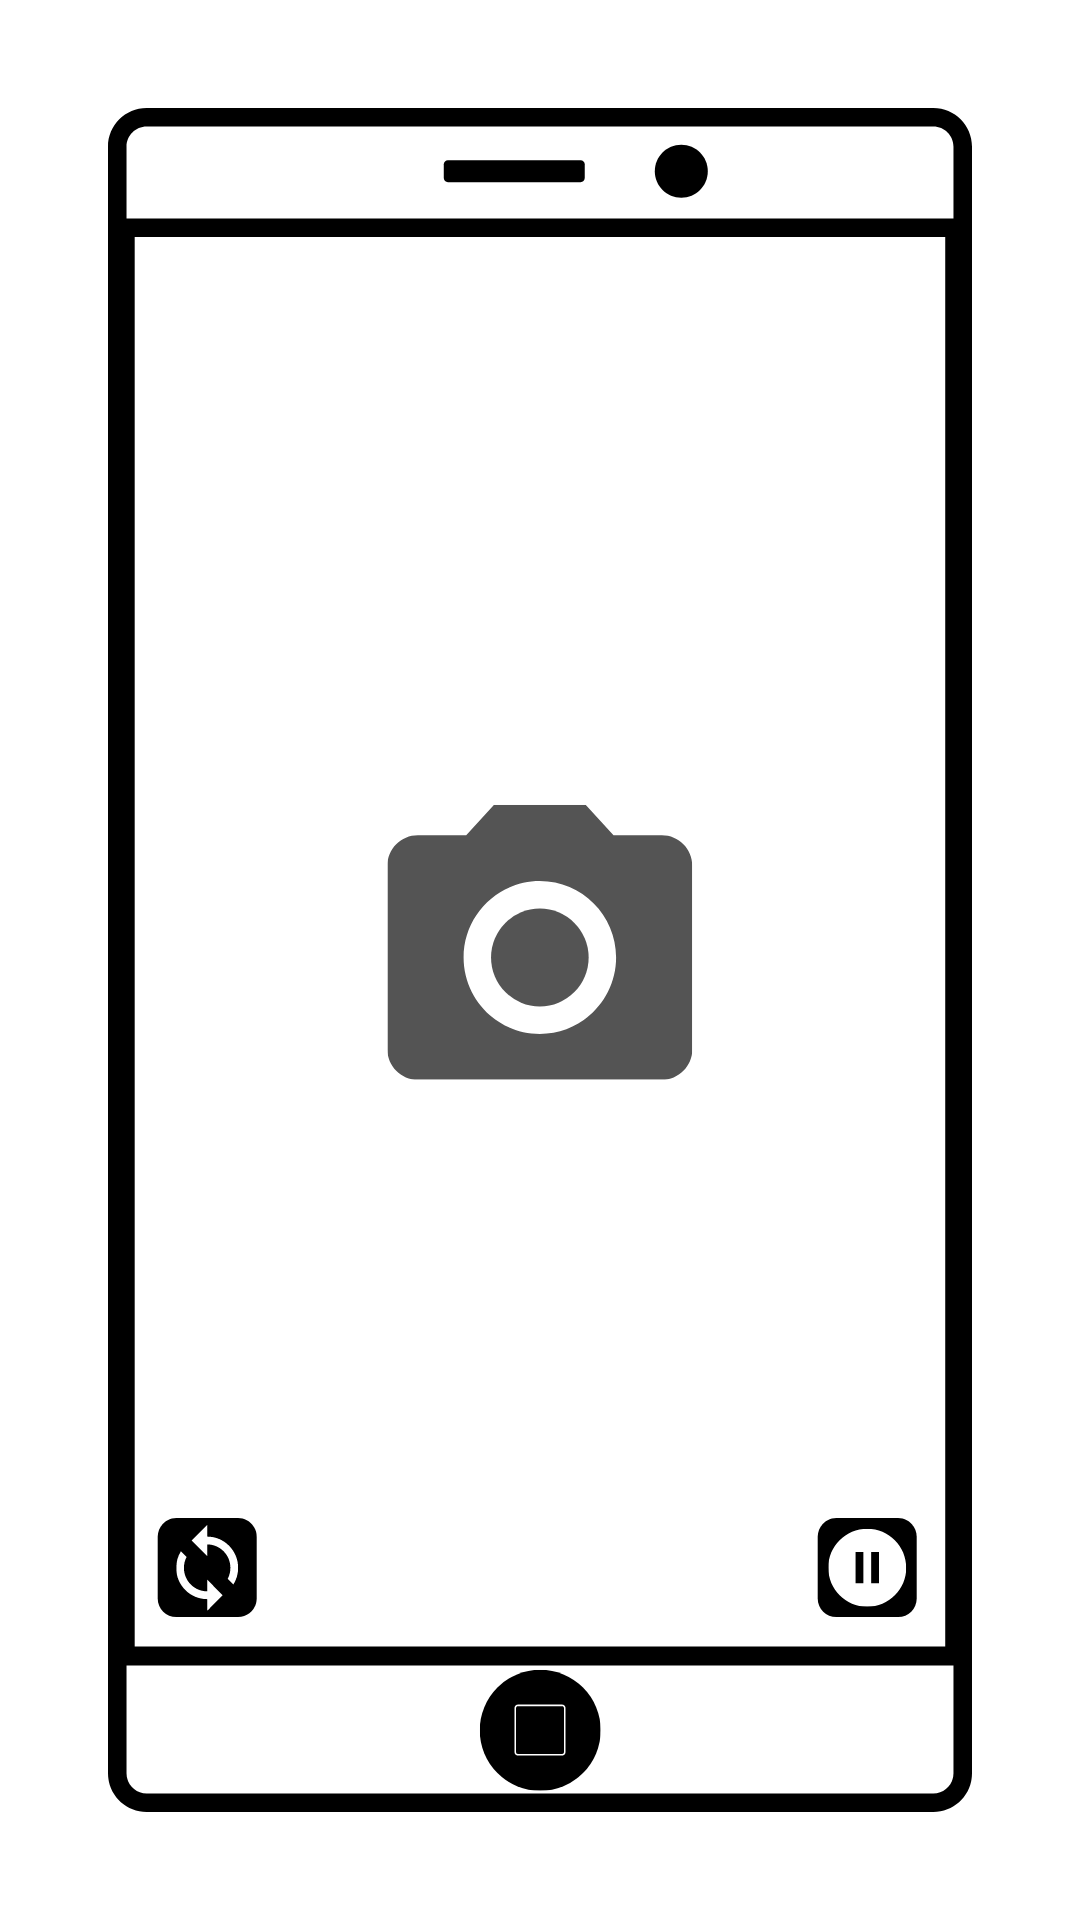
\includegraphics[scale=0.25]{appMockup.png}
\newline
Our application will deliver all of its content through AR, therefore, the mockup can only depict what the AR viewport will look like.

\section{Use Cases}
This section presents detailed use cases of our system.

\section{Datasets}
Not Applicable.

\section{System Diagram}
This diagram gives a high-level view of the different components of our system and the interactions between them. Each component and the particular tools/technologies/libraries used to build it are described.